\renewcommand\thechapter{\Roman{chapter}}
\chapter{DESARROLLO} \label{ch:desarrollo} \thispagestyle{fancy}
\renewcommand\thechapter{\arabic{chapter}}
%%%%%%%%%%%%%%%%%%%%%%%%%%%%%%%%%%%%%%%%%%%%%%%%%%%%%%%%%%%%%%%%%%%%%%%%%%%%
En este capítulo se describe el desarrollo del diseño para la implementación del laboratorio virtual. Se muestra el diagrama de flujo a seguir para llevar a cabo la programación y como es que va a funcionar. Finalmente se presenta la etapa que se esta siguiendo, con un robot de 3GDL el cual es realizar un simulador básico para poder comprender las características que se debe de tener.

\newpage
\begin{figure}[!h]
\centering
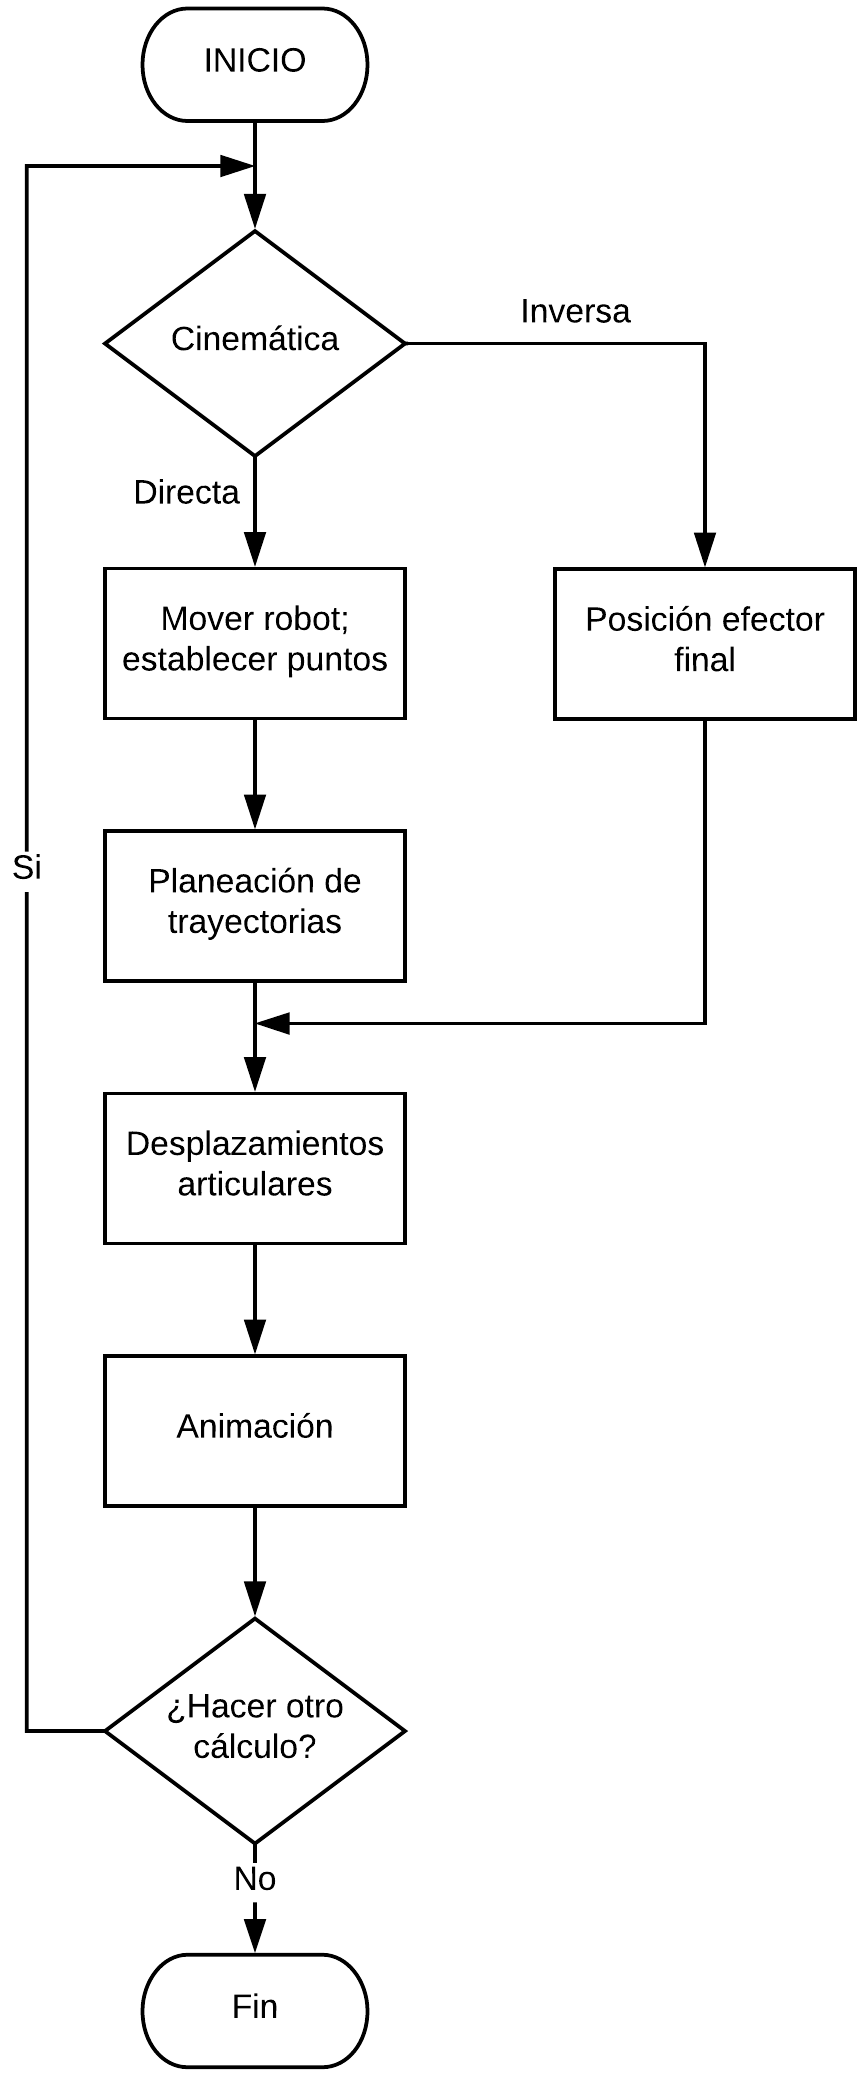
\includegraphics[width=0.45\textwidth, height=0.75\textheight]{./figs/diagramaprogramacion}\\
\caption{Diagrama de flujo para la programación}
\label{diagramadeprogramacion}
\end{figure}

En la figura \ref{diagramadeprogramacion} se quiere iniciar con un menú el cual despliegue dos simples opciones, una la cual va a llevar al cálculo de la cinemática directa y otro de la cinemática inversa, según la opción que se seleccione en este caso si fue la directa se mostrará un menú el cual permita posicionar las articulaciones de manera libre, a continuación realizará una planeación de trayectorias para ejecutar los cálculos necesarios y que pueda hacer los desplazamientos articulares mostrándolos mediante la animación; mostrará un menú el cual permita seleccionar si se desea finalizar con el programa o desea continuar con otro cálculo; se podrá continuar con la cinemática inversa el cual consta de posicionar el efecto final, el programa ejecutará los cálculos para poder hacer los desplazamientos articulares mostrándolos como se menciona anteriormente con su respectiva animación; de igual forma muestra el menú para continuar con otro calculo, de no ser así se finaliza el programa.\\

La etapa en la que se encuentra el proyecto es en base a un programa con el cual podemos crear un ambiente virtual que el mismo Matlab trae integrado es ir experimentando como posicionar piezas en un espacio, ensamblarlas, etc. 
Para que se logre crear un menú de igual forma con un comando el cual nos abrirá una ventana que se tiene que posicionar botones, sliders, etc; se necesita crear un link entre el panel creado y el robot en 3D es la etapa en la cual está el proyecto para poder finalmente interactuar con él.\\
Como se mencionó anteriormente dentro de Matlab se encuentra una herramienta llamada V-Realm Builder la cual permite crear desde figuras básicas o abrir diseños creados en CAD, en este trabajo se obtuvo un brazo robótico en SolidWorks, guardando la pieza en un formato de archivo .wrl se puede abrir en el programa dicho anteriormente, al abrirlos se deberán colocar en un punto del espacio mediante coordenadas hasta terminar formando la figura.\\
En la ventana de comandos de MatLab mandando llamar ``GUIDE'' abrirá otro menú el cual permite crear un panel con botones igual se puede personalizar con colores y las posiciónes de los sliders, títulos, botones, etc.\\
Al finalizar el archivo .gui el cual se genera de la extensión ``GUIDE'' crea un código el cual se deberá modificar en cuanto a las características del archivo .WRL que tenemos del robot.